
\section{The cloud computing}

In the 1980s, people were used to play music with their tapes and then with their Cd player. Everyone wanted to own his assets. It was the same thing from the 2000s with computers. It was typical for every family to possess an imposant computer and to buy an extra hard disk to store music, movies, and pictures. It's the same way for companies, working with significant amount of data or ones wanting to create websites for a lot of customers. This is the way our society was designed. Today, things get different. People just want to consume services. They don’t care about possessing the real object since they always can get the services. Due to this change of menthalies, when the number of internet consumers were growing, it became a crucial need for every company working in I.T (Informatic Technologies) to be able to create online applications, able to return a response to each request. This is why services like \textbf{IaaS} were born.

\subsection{IaaS: Infrastructure as a Service}

This purpose of this model is to give companies the opportunity to manage and deploy services remotely. By the way this create the illusion of infinite computing on demand. In the Iaas model, only the hardware is exported remotely. Thus any startup or big group can store their data remotely. It does not need to own a server anymore. This model gives the possibility to access to the server capability remotely without caring about the monitoring and the scalability. While companies don't need to own their servers, that give us the possibility to pay for hardware only for a short period. This service is also called: Utility Computing. Nowaday, Amazon Web Service (Amazon WS) is one of the greatest leader on this service. However, when thinking about scalability and high availability, the hardware part is not always enough. The middleware or software also needs to be scalable. Further on, developers do not ever manage all the operating system installed on the machine. This is why we also talk about \textbf{PaaS}.

\subsection{PaaS: Platform as a service}

With Paas, users can run their environment, build and compile without worrying about the infrastructure and the OS (Operating system). Here some examples of Paas provider: Google app engine, Windows Azure, Amazon web services, Digital Ocean… etc.  Usually, the developers only need to choose their computation power (CPU, RAM) and choose their operating system before to get started deploying their solution. However, users are constraints to the provider's infrastructure and migration issues. On the other hand, they also can expose their product easier and more quickly than they used to, without thinking about the scalability and the high availability. This model will unleash a wave of new services know under the name: \textbf{SaaS}.

\subsection{SaaS: Software as a service}

Software as a service is a model that offers on-demand paiement for software applications  to users. People don’t need to install the software on their computer anymore. There is only a single instance of the software which is stored online. SaaS is an on-demand service where the user doesn't buy a license to install but pay depending on his usage. We call this: \textbf{Pay-as-you-go}. Being able to deploy services for thousand or millions of users gives companies the possibility to decrease the price of services. While the cost is reduced, customers are more and more able to purchase the product. Then, companies can again drop the price of the software (Supply and demand model). Users can access the product everywhere from any platform, which is perfect for collaborative work (Office 365, Github, Gitlab and so on). This model also gives a lot more flexibility. It gave the possibility for any user to try a service. If he doesn't like it, he can just throw it away and take another service. By the way, this model seems well suited to fit our consumer society.
\newline

\begin{figure}[H]
  \centering
  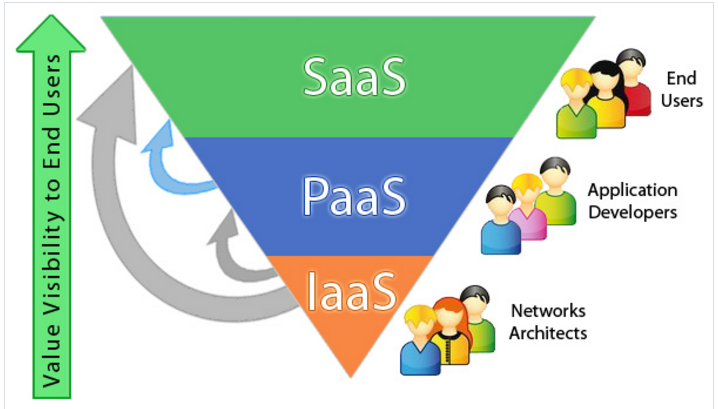
\includegraphics[width=8cm]{body/tri.png}
  \caption{Image from aboutcloudservice.com}
\end{figure}

Finally, datacenters (composed of hardware and software) are what we will call the \textbf{Cloud}. The public cloud is what is cell/rent to the public while the private cloud is only what is referred to internal datacenters of big groups (providers or not). But more importantly, the sum of SaaS and \textbf{Utility computing} (which do not include private cloud) is called the \textbf{Cloud Computing}.

\subsection{Some usage of Cloud Computing}

For the final users, cloud computing can be used in several and different ways. Nowadays, we can use services to store Photos and media and access it anywhere any time. While accessing features like Auto synchronization (from the phone to the cloud), Auto-Album generation, auto-filtering and so on. Cloud computing has also changed the way we are watching movies/series online because we don't need to own DVDs as before. Everything can be accessed online and the leader in this fields is currently Netflix. The growing of cloud computing also changed the way companies are working every day. Instead of using simple email platform, new services give the opportunity to chat with other workers on the same project, directly online. One of the newest services is Slack which is a SaaS. Moreover, the way people are using their computational capability is changing. Previously, only companies rented remote CPUs or GPUs power. Nowadays, gamers are using remote GPU to play games with an intensive workload while all the graphics computation is export remotely. Thus, anyone can play fantastic video games without possessing a big computer. We are also going to talk in the last part of this article about an other way to export the computation. But this time, for artificial intelligence computation.

\section{Cloud providers}

\subsection{Digital Ocean}

Digital Ocean is a cloud computing service designed for developer. In other words, it’s a PaaS provider.

\subsubsection{Global user experience}

Digital Ocean commonly used their VPSs under the name: \textbf{Droplets}. Before to use one, the client needs to select a predefined operating system which can be configured with a vast range of options. However, it is not possible to set up the operating system. Once the droplets have been deployed, the client is free to install anything he wants on the server (Web Application, API, Gaming server and so on). Also, any droplet can easily be transferred from one server (For instance, in America) to another server in the world. Also, let’s say a front-end developer would like to deploy a WordPress server without much knowledge about the Linux kernel. Digital ocean give the possibility to create a “One click” droplets in few minute with WordPress installed on. This is the same for others application like: Gitlab, Django, LEMP, Docker and so on. Theses services come with a simple control panel which allows any user to handle their droplets without a deep understanding of either the hardware or the architecture or even without any system administration knowledge.

\subsubsection{What’s under the hood ?}

Their servers are only composed of \textbf{SSD} (solid-state drive), which is fantastic for fast I/O access. Of course, Digital ocean is engineered with powerful servers. Multiples VPS (Virtual Private Servers) are installed on each of them to allocate a subpart of the server computation/storing. Thus, each VPS could be used with root access, and each client can install and do whatever he wants.  Digital Ocean used powerful Hex Core machines with dedicated \textbf{ECC Ram} and \textbf{RAID SSD}. Each droplets working on the servers are using \textbf{KVM virtualisation} which stands for Kernel-based Virtual Machine. This architecture is one of the most efficient ways to handle lots of virtual machine in parallel, the whole, with security and effortless control. This structure also allows a private network; It is used by droplets to transfer information within each other without consuming the monthly bandwidth.

\subsubsection{Conclusion}

In conclusion, what makes Digital Ocean a reliable alternative as a cloud provider, is his ability to provide quick access to a virtual online machine with a minimum of knowledge and a user-friendly interface. The whole can be saved, removed, exported and restored easily on a new server. All these points responds to the consumer society we told earlier in this document.
\subsection{Amazon WS}

My first feeling when I tasted out amazon WS after having dived into Digital Ocean, is the complexity of the platform. Surely you may need slightly more knowledge or time to understand how Amazon WS works. In fact, you have access to a large collection of services available from many groups of servers/regions for high availability and low latency applications. You can find services with highly durable storage, low-cost computer, both managed and unmanaged databases, led and unmanaged servers, and of course, high-level functions with pre-installed web applications (Wordpress, Drupal…). In fact, Amazon WS can be viewed  as a provider of both IaaS and a PaaS.

Example of customers using Amazon WS:

\begin{itemize}
    \item \textbf{Pinterest}: With over 410 terabytes and a small engineering team, amazon is the perfect way for us to access to a scaled server with high availability.
    \item \textbf{Netflix}: One of the most popular websites in the world.
    \item \textbf{Reddit}: With only 20 employees, it was impossible to manage their physical server. By migrating to Amazon they can have scaled websites with 4 billion page views per month.
\end{itemize}

\subsubsection{Architecture}

To handle this significant amount of users, Amazon used auto-scaling. This is a way to provide a computation capacity watching precisely the user demand. But how does auto-scaling works ?

\textbf{Auto scaling}

\begin{figure}[H]
  \centering
  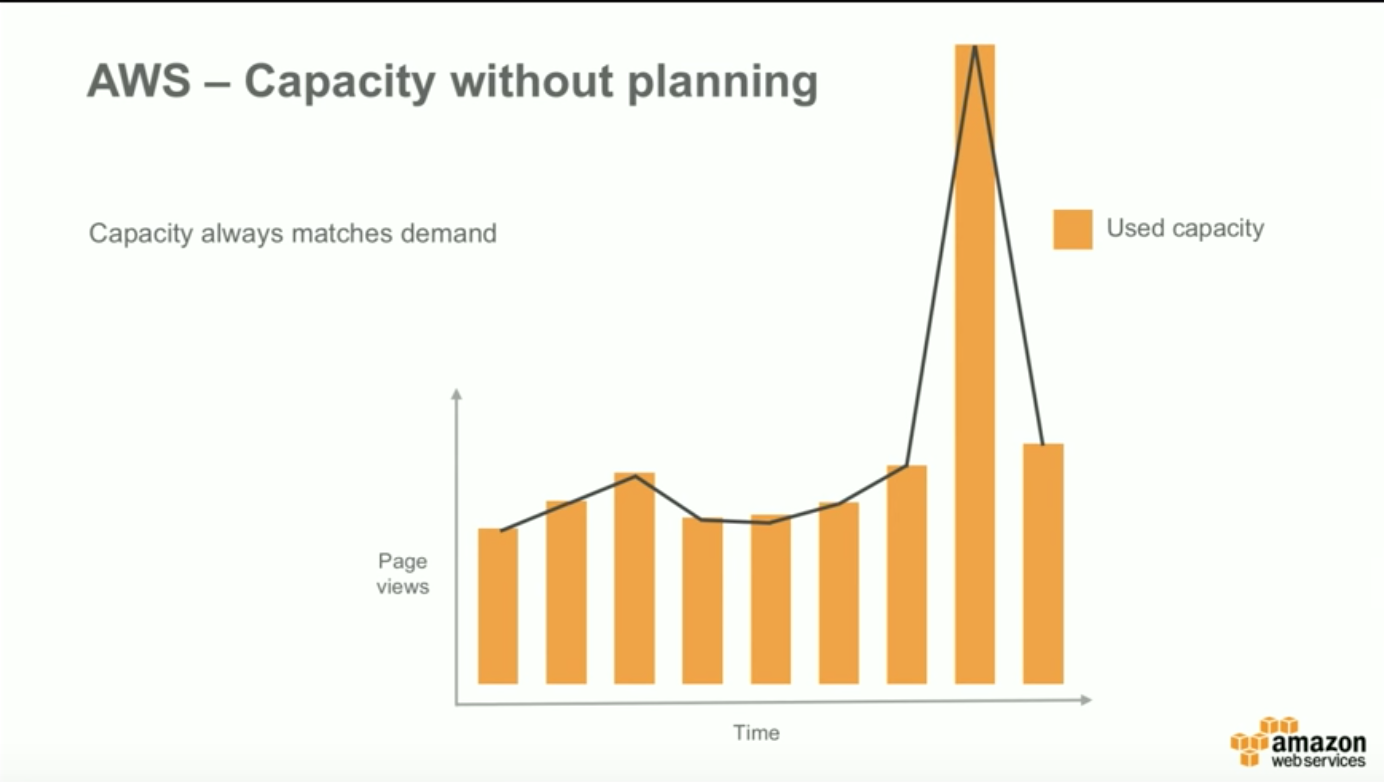
\includegraphics[width=8cm]{body/scale.png}
  \caption{Image from Amazon WS slides}
\end{figure}

\begin{itemize}
    \item \textbf{Elastic Load Balancing} which distributes the traffic across multiple channels. In fact, load balancing can be configured within a Ngnix or Apache server for instance. But by using amazon server, almost no management is involved.
    \item \textbf{EC2 AutoScaling Group} is one service  allowing to scale from 1 instance  of your application, up to 100 instances depending on your configuration (CPU Usage, pages loaded or even custom metrics)
    \item \textbf{Elasticache for Memcached}: It is a simple tool, used to handle issues, relative to significant bulk of cache.
    \item \textbf{Multi-AZ RDS}: Relational database well suited for the cloud, make it easy to setup up, operate and scale database.
\end{itemize}

\textbf{Hardware customization}

By using Amazon, you can not only access to a small amount of software services but also change and replace your hardware stuff. In fact, working with Amazon WS is like working with lego blocks that you can assemble quickly to support any workload.

\section{Next to the cloud}

By building necessary infrastructure, we are now able to support millions of devices connected to internet at the same time. In fact, internet is just a set of protocole (HTTP, TCP, UDP, FTTP) guiding how to transfer data. However, the most commun used protocole is  HTTP (Hyper Text Transfer Protocol). Developed by Tim Berners-Lee in 1989, we are still using this protocol on the web, almost thirty years later. Any user of internet, sends requests (GET, POST, PUT, DELETE…) before getting a response from the server. However, there are some downsides:

\begin{itemize}
    \item The first one is \textbf{Bandwidth}: As we saw above, the architecture of providers are well suited to support huge amount of requests. In reality, every days, every hours, servers get down because of the number of users whom would like to connect to internet.
    \item The second problem is \textbf{Latency}. We can try to increase the transfer speed, but only until a given point where it will be not possible any more. Centralizing data into remote datacenter inevitably reduce availability by increasing latency. In fact, the only solution is to move data closer to the user. And this is what cloud providers are doing. But sometime, it is not enough. \textit{“In recent years, there has been a strong push to move everything to a centralized cloud, enabled by virtualization and driven by the need to cut costs, reduce the time to market for new services, and increase flexibility. In the process, we lost sight of how important the location of functionality is to performance, efficient use of network resources and subscriber experience. Physical distance inevitably increases latency.”} Monica Paolini.
    \item Then, the third problem is \textbf{resiliency}, Unless one particular data is saved in two place, if one cloud provider is hack, data is lost.
    \item Finally, and I think this is the most important: \textbf{Centralization}. By letting company keep care of our data, we can’t be sure of how our data is used. We can’t be sure to protect our privacy.
\end{itemize}

I will talk about two close solution. \textbf{Fog computing} and \textbf{IPFS}.

\subsection{Fog computing}

In computer science, Fog computing is related to an architecture that extends services offered by the cloud to edges devices. Edges devices are composed of all devices able to receive an internet connection. From many points of view, fog computing is seen as the new cloud and from others, it is only an extension. My thoughts about this are the following: it is neither one nor an other. It’s both. Fog computing would not exist without cloud and cloud would be better with fog.

For instance, Consider two scenarios. One using Cloud computing, the other one using Fog Computing.

\begin{figure}[H]
  \centering
  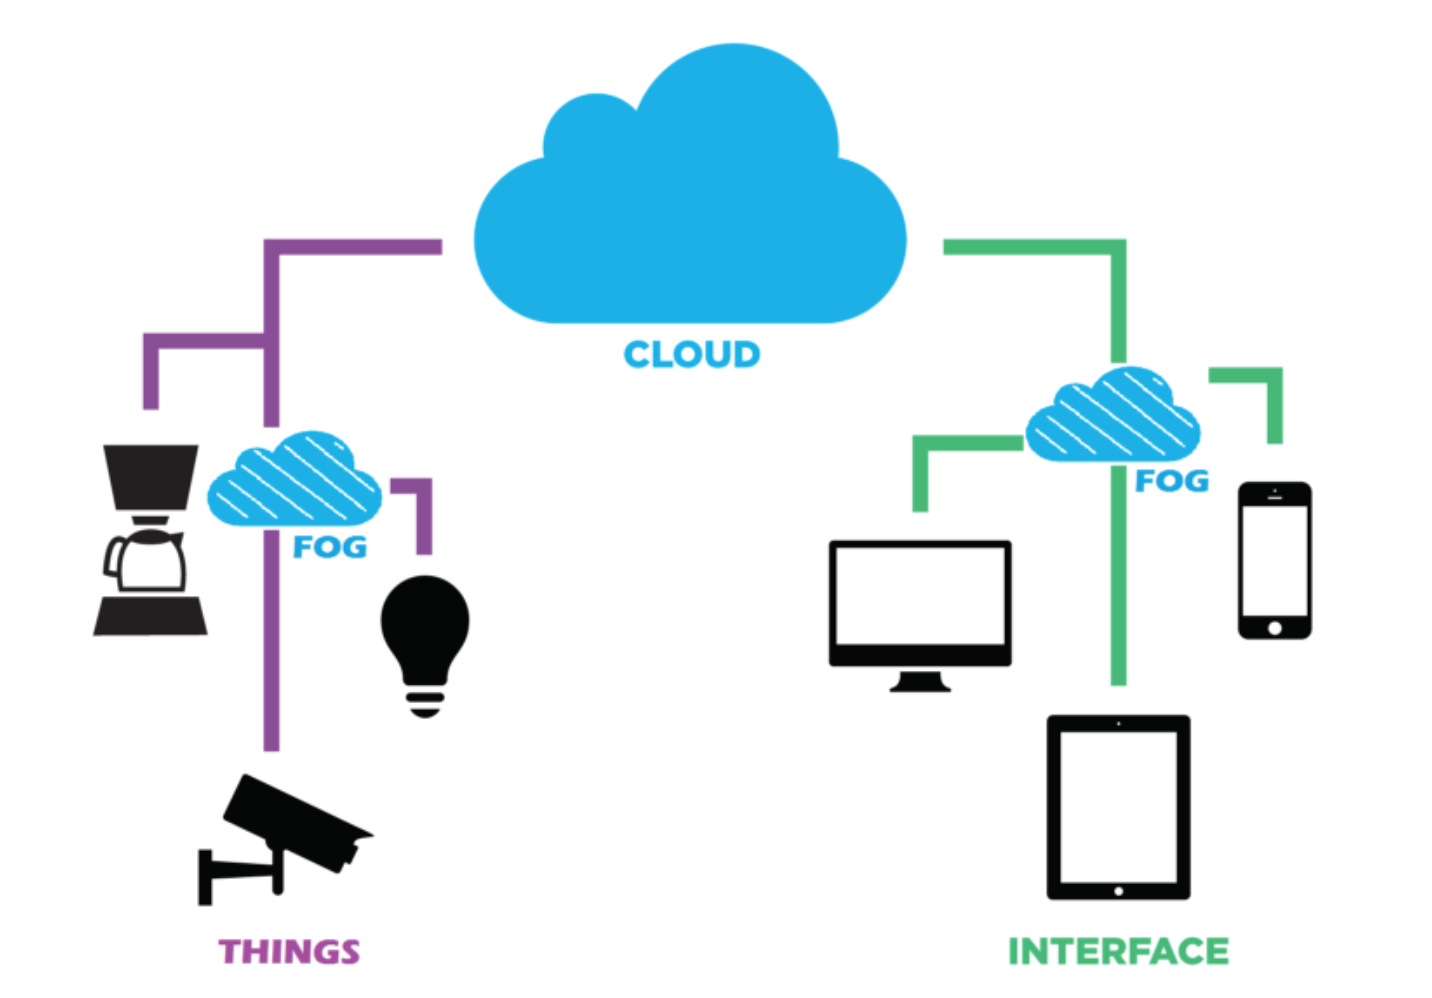
\includegraphics[width=8cm]{body/fog.png}
  \caption{Image from openfogconsortium.org}
\end{figure}


\subsubsection{With cloud computing}

A person landing to Paris airport, may wants to book a taxi using his smartphone. There are about 400 hundreds taxi near to the airport waiting for a notification on their phones. Using the simple cloud model, each traveler (Let’s say 250) will send their data to the cloud while  400 taxi will still ping the server for a new client. At scale, the bandwidth to push all this data to the same server is really inefficient knowing all theses phones are located at the same airport.
\subsubsection{With fog computing}

Using this model, each traveler’s phone in the airport will now compute the most efficient way to send data to the nearest taxi phone in the airport. The data go through each local node (each devices is a node) before reaching its destination. Thus, fog node can extends the role of the cloud by exporting some part of the computation between devices in the same place.

\subsection{Users of Fog computing}

Over the last months, companies  like Amazon, Microsoft and Google have announced their ambitions to take part in fog Computing. However, in order to democratise this model into the whole community of cloud providers and   inside the software embedded in each devices will take some times. However, since november 2015 the Openfog Consortium are working with academia and researchers to make fog computing fully working and part of cloud computing.

\subsection{IPFS}

IPSF was created to solve the two problems we talked above about centralisation and resiliency. IPFS is a new protocol coming with the movement of fog computing. The aim of this protocol is to makes data accessible at any time without entity controlling our data.

\textbf{How doest IPFS works ?}

This protocol is based on content address while HTTP is based on IP Address. Thus, each file have a unique fingerprint called \textbf{cryptographic hash}. It means that when you take your phone to request an image, a video or any content, the transfer will not be processed between your and a server, but between you and the closest node (This node can be an other phone close to you). Moreover, the data can be transfered byte per byte using not only one node, but multiple ones. In fact, IPFS is based on peer-to-peer protocol with \textbf{distributed hash table (Chord)}. Inspired by the git protocol, this method can remove files duplications and tracks version history for every file. Thus, data is encrypted using a data structure call \textbf{merle dag} as well as the Git protocol. For more information about the exact structure, checkout the white paper of Juan Benet (References).

\section{Artificial intelligence’s Impact on Cloud Computing}

In this section, we are going to dive into how providers could benefit from Artificial intelligence (A.I) wave proposing new services. Back to 10years from now, the symbolic A.I was the most used. However, in the past few years, thanks to the growth of computer capability, it became simple to use optimisation based techniques.

\subsection{Machine learning and Deep Learning}

The machine learning is a subpart of A.I including techniques like clustering, supervised learning, unsupervised learning and so on. A part of these methods is based on the algorithm of \textbf{Gradient Descent} to optimise an objective function. By optimizing a given function, we can train a model to predict some output (the prediction) given some input (the features). While machine learning is based pre-compute features, Deep Learning adds others techniques (Multiples layer of abstraction) to be able to deduce essential features by itself. For instance, let’s say we would like to train a model capable of recognizing cat pictures. A machine learning model would first try to detect pattern such: eyes, nose, ears, the month of the cat using image processing methods and then build a machine learning classifier. A deep learning model does not need such features, it is possible to fit the model with rows pixel of images and let the model build is own representation of a cat by itself. The latter works better. But what is the relationship between cloud computing and deep learning?

\subsection{Computation capability problems}

Thank the growing of computer capability, deep learning became possible. Nowadays, almost everyone is able to launch simple deep learning model on their laptops. But that’s the point: it is only simple deep learning models. Anyone who would like to go more in-depth (Convolution Neural network for instance) by using such advanced techniques would be stuck by his CPU (Central Processing Unit) capability. How to solve the problem?

\begin{itemize}
    \item The solution would be to buy a good \textbf{GPU} (Graphics Processing Unit). Indeed, GPU is more suited to handle big vector and matrix product than CPU, and deep learning is all about matrix product. But as we said earlier in this document, people don’t care about owning the object as long they can access to the service. We use this insight to dive into the next solution.
    \item Exporting the models remotely. By uploading a model to the cloud, it would be possible for everyone to train substantial deep learning model without GPU. Thus, this avail to democratize artificial intelligence by creating new services on the cloud.
\end{itemize}

\subsection{The new service}

This new service is already available online on such platforms like Amazon WS, Google cloud which let the user choose a fit server with a GPU. However, this service is often expensive and not always accessible to everybody. The challenge for the next years would be to downgrade the price of this kind of server and to let it available in more location in the world. Upload the model do not need a lot of bandwidth, however, uploading the dataset able to train the model take a certain amount of time. The closest the server would be, the fastest the training of the model could start. New providers like FloydHub try to create new ways of handling these problems, by creating “disposable severs”. Any developer can launch a training on one server and pay only for the period of training. This is a whole new kind of business model which gives the possibility to users to pay less for the same service.

\section{Conclusion}

To summarize, cloud computing has changed many things in the way people and companies live every day, whether we are working in a company or we are only using phone applications. The way software is designed has radically changed during the past few years. However, I am really convinced that this is only the beginning. The cloud computing needs to evolve again in order to really fit our society. This is why new approaches like Fog computing should be considered.
